\documentclass[runningheads]{llncs}

\usepackage{float}
\usepackage{graphicx}
\usepackage{xcolor}

\newcommand{\todo}[1]{\textcolor{red}{\textbf{TODO}: {#1}}}

\begin{document}

% Please feel free to suggest a better title
\title{An Assurance Pattern for Cyber-Resilient Systems Engineering}

\author{
	Isaac Amundson\inst{1} 
	\and Darren Cofer\inst{1} 
	\and David Hardin\inst{1} 
	\and John Hatcliff\inst{2}}

\institute{
	Applied Research and Technology, Collins Aerospace, USA \\
	\email{\{isaac.amundson,darren.cofer,david.hardin\}@collins.com}\\
	\and Kansas State University, USA \\
	\email{hatcliff@ksu.edu}
}

\authorrunning{I. Amundson et al.}

\maketitle

\begin{abstract}

On the DARPA Cyber Assured Systems Engineering (CASE) program, our team has developed BriefCASE, an open-source model-based engineering environment for cyber-resilient system design.  BriefCASE is comprised of tools that emit evidence of correctness that is maintained by the framework and can be used to substantiate assurance claims.  
In this paper, we describe a comprehensive cyber-resiliency assurance pattern, which BriefCASE instantiates with the system under development. Evidence collected by the framework is automatically evaluated in the resulting assurance case to determine whether cyber-resiliency goals have been acceptably satisfied.

\end{abstract}

DISTRIBUTION STATEMENT A. Approved for public release: distribution unlimited.

% Include short CASE / BriefCASE overview
\section{Introduction}
\label{sec:introduction}

% DARPA CASE

% REPHRASE THIS PARAGRAPH TO AVOID COPYRIGHT CONCERNS
%\todo{Rephrase first paragraph - copied from MODELS paper}
%
%In recent years, aerospace stakeholders have realized that avionics systems are subject to possible cyber attacks just like other cyber-physical systems. Thus, in addition to being fault tolerant, safety-critical avionics systems must also be cyber-resilient. Cyber-resiliency means that the system is tolerant to cyber attacks just as safety-critical systems are tolerant to random faults: they recover and continue to execute their mission function, or safely shut down, as requirements dictate. Unfortunately, systems engineers are currently given few development tools to help answer even basic questions about potential vulnerabilities and mitigations, and instead rely on process-oriented checklists and guidelines. Cyber vulnerabilities are often discovered during penetration testing late in the development process; or worse yet, they may be discovered only after the product has been fielded, necessitating extremely expensive and time-consuming remediation. This is not a sustainable development model. 

The DARPA Cyber Assured Systems Engineering (CASE) program is targeted at developing tools for design, analysis, and verification that enable systems engineers to \textit{design-in} cyber-resiliency for complex cyber-physical systems. 
%
% BRIEFCASE TOOLS AND FEATURES
Our team developed BriefCASE~\cite{case-at-scale}, a tool chain for developing and assuring cyber-resilient embedded systems according to the CASE workflow depicted in Fig.~\ref{fig:workflow}. BriefCASE provides a development environment for modeling system architectures in AADL~\cite{feiler-aadl}, analyzing the models for cyber-vulnerabilities, mitigating those vulnerabilities by applying automated model transformations, formally verifying security properties in the model, generating high-assurance component code from model specifications, building the system to a secure kernel target, and finally, generating a system cybersecurity assurance case.  

\begin{figure}[h] 
	\centering 
	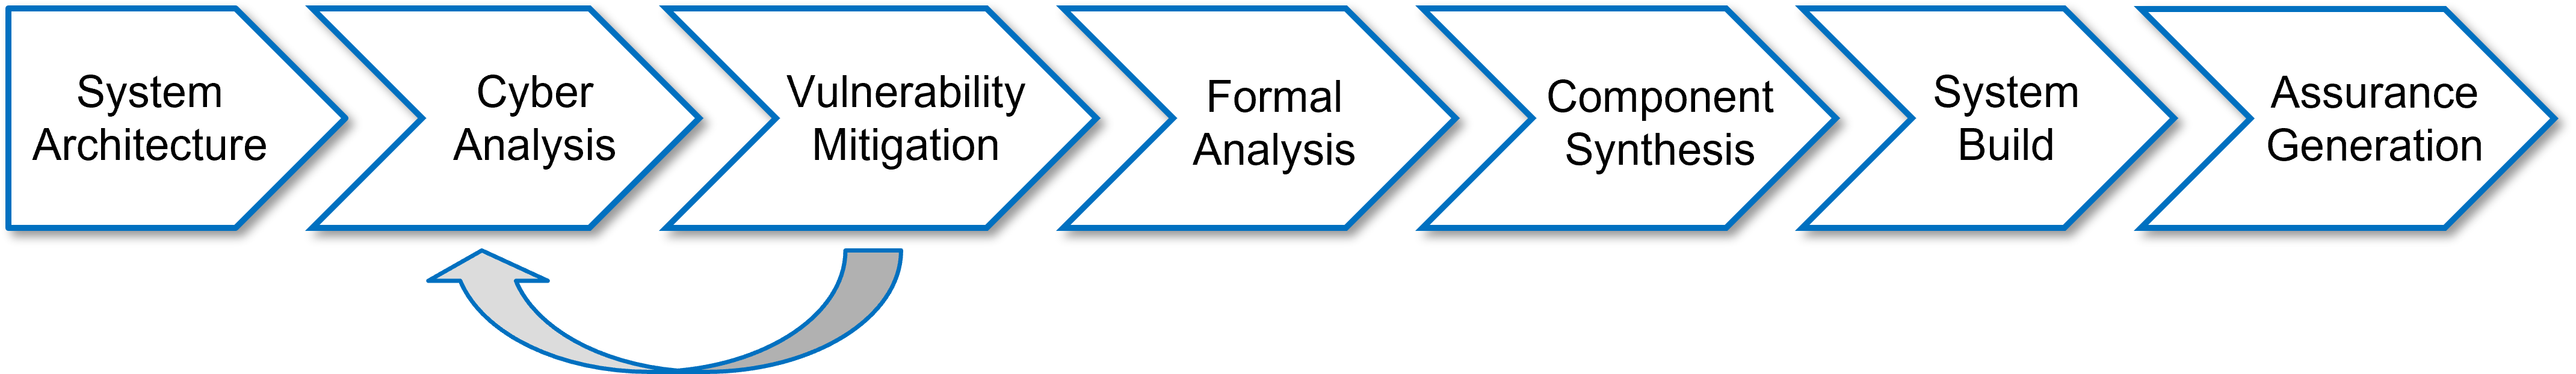
\includegraphics[width=\textwidth]{figs/workflow.png}
	\caption{Cyber Assured Systems Engineering workflow.}
	\label{fig:workflow} 
\end{figure}

% ASSURANCE
For the development of high-assurance products, there are multiple stakeholders that must be convinced of the product's dependability prior to deployment.  First and foremost, the product developer must be confident that the product operates correctly with respect to the intent of the specification.  Next, the certification or accreditation authority (where applicable) must be convinced.  Finally the customer, end user (and often other stakeholders in between) will need to be convinced the product will behave as intended.  Assurance is the process by which an organization compiles a comprehensive argument to demonstrate a product's dependability~\cite{???}.  In order to be effective, the argument must be well-formed, complete, and substantiated with evidence.  
%
Assembling such an argument is not a straight-forward task.  For heavily-regulated environments, it is argued that construction of these arguments should never be left to automation~\cite{???-Holloway}.  In other situations, arguments can be constructed based on assurance templates, or \textit{patterns}, in which generic arguments are defined (ideally arrived at through consensus by a body of experts), then instantiated with a concrete system instance.  This is the approach taken by BriefCASE, which includes a cybersecurity assurance pattern that is instantiated with the system under development, and incorporates evidence produced by artifacts generated by the framework workflow.

Patterns for assurance case argumentation have been considered in~\cite{Denney13:pattern}, \cite{Hawkins11:pattern}, \cite{Kelly97:patterns}, and~\cite{Sun11:pattern}. An approach to apply and evolve assurance cases as part of system design is found in~\cite{Graydon07:dev}, which is similar to the process we use in BriefCASE.
%
In previous work~\cite{resolute-destion}, we described assurance pattern fragments corresponding to specific BriefCASE vulnerability mitigations.  However, those patterns primarily focused on assuring that aspects of security requirements were satisfied in the model by examining the model structure (for example, demonstrating that an inserted filter component could not be bypassed).  
%
% CONTRIBUTION AND PAPER OUTLINE
In this paper we expand on that work by presenting a more comprehensive CASE assurance pattern covering the generation and ingestion of cyber requirements, requirement satisfaction in the model and requirement satisfaction in the realization of the model.  

% RELATED WORK (Assurance patterns, assurance generation, ARCOS?, DMILS, VERDICT, DESTION, what's new here)
\todo{Describe and compare with D-MILS, VERDICT}

The high-level structure of our CASE assurance pattern is inspired by the D-MILS argument pattern~\cite{dmils}, in which system dependability properties are assured via modules arguing component, compositional, and implementation correctness.  

VERDICT~\cite{verdict} is a framework also developed on the CASE program with some similarities to BriefCASE.  Although VERDICT does generate and evaluate assurance arguments based on analyses performed as part of the tool workflow, the assurance arguments are only shallow fragments of a comprehensive cybersecurity case.

In Section~\ref{sec:briefcase}, we present an overview of the BriefCASE tool chain and workflow. Section~\ref{sec:assurance-pattern} describes our assurance pattern with respect to the CASE workflow. Specifically, we focus on arguments for security requirement correctness, model correctness, and implementation correctness.  We provide concluding remarks and discuss future directions in Section~\ref{sec:conclusion}.


% Section 1: CASE description 
% Be specific about differences with D-MILS
% Section 2: Description of Briefcase workflow
% Section 3: Walk through assurance pattern


% Include DMILS - compare/contrast
% Integrate this section with Intro if short on space
%\section{Related Work}
%\label{sec:related-work}
%


\section{Cyber Assured Systems Engineering with BriefCASE}
\label{sec:briefcase}
% BriefCASE tool overview
BriefCASE is predicated on a Model-Based Systems Engineering (MBSE) process, in which models are the primary vehicle for communication and understanding among the parties tasked with designing the system. 
It is implemented as a collection of plugins in the Eclipse-based Open Source AADL Tool Environment (OSATE), the reference AADL modeling tool. In this section, we describe the tools that comprise BriefCASE, as well as the built-in mechanism for automated assurance generation.  Additional information on BriefCASE can be found in~\cite{case-at-scale}.

\subsection{BriefCASE Architecture}

The BriefCASE architecture (see Fig.~\ref{fig:briefcase-architecture}) starts with the development of a baseline AADL model of the system. BriefCASE is implemented as a collection of plugins in the Eclipse-based Open Source AADL Tool Environment (OSATE), the reference AADL modeling tool. 

\begin{figure}[h] 
	\centering 
	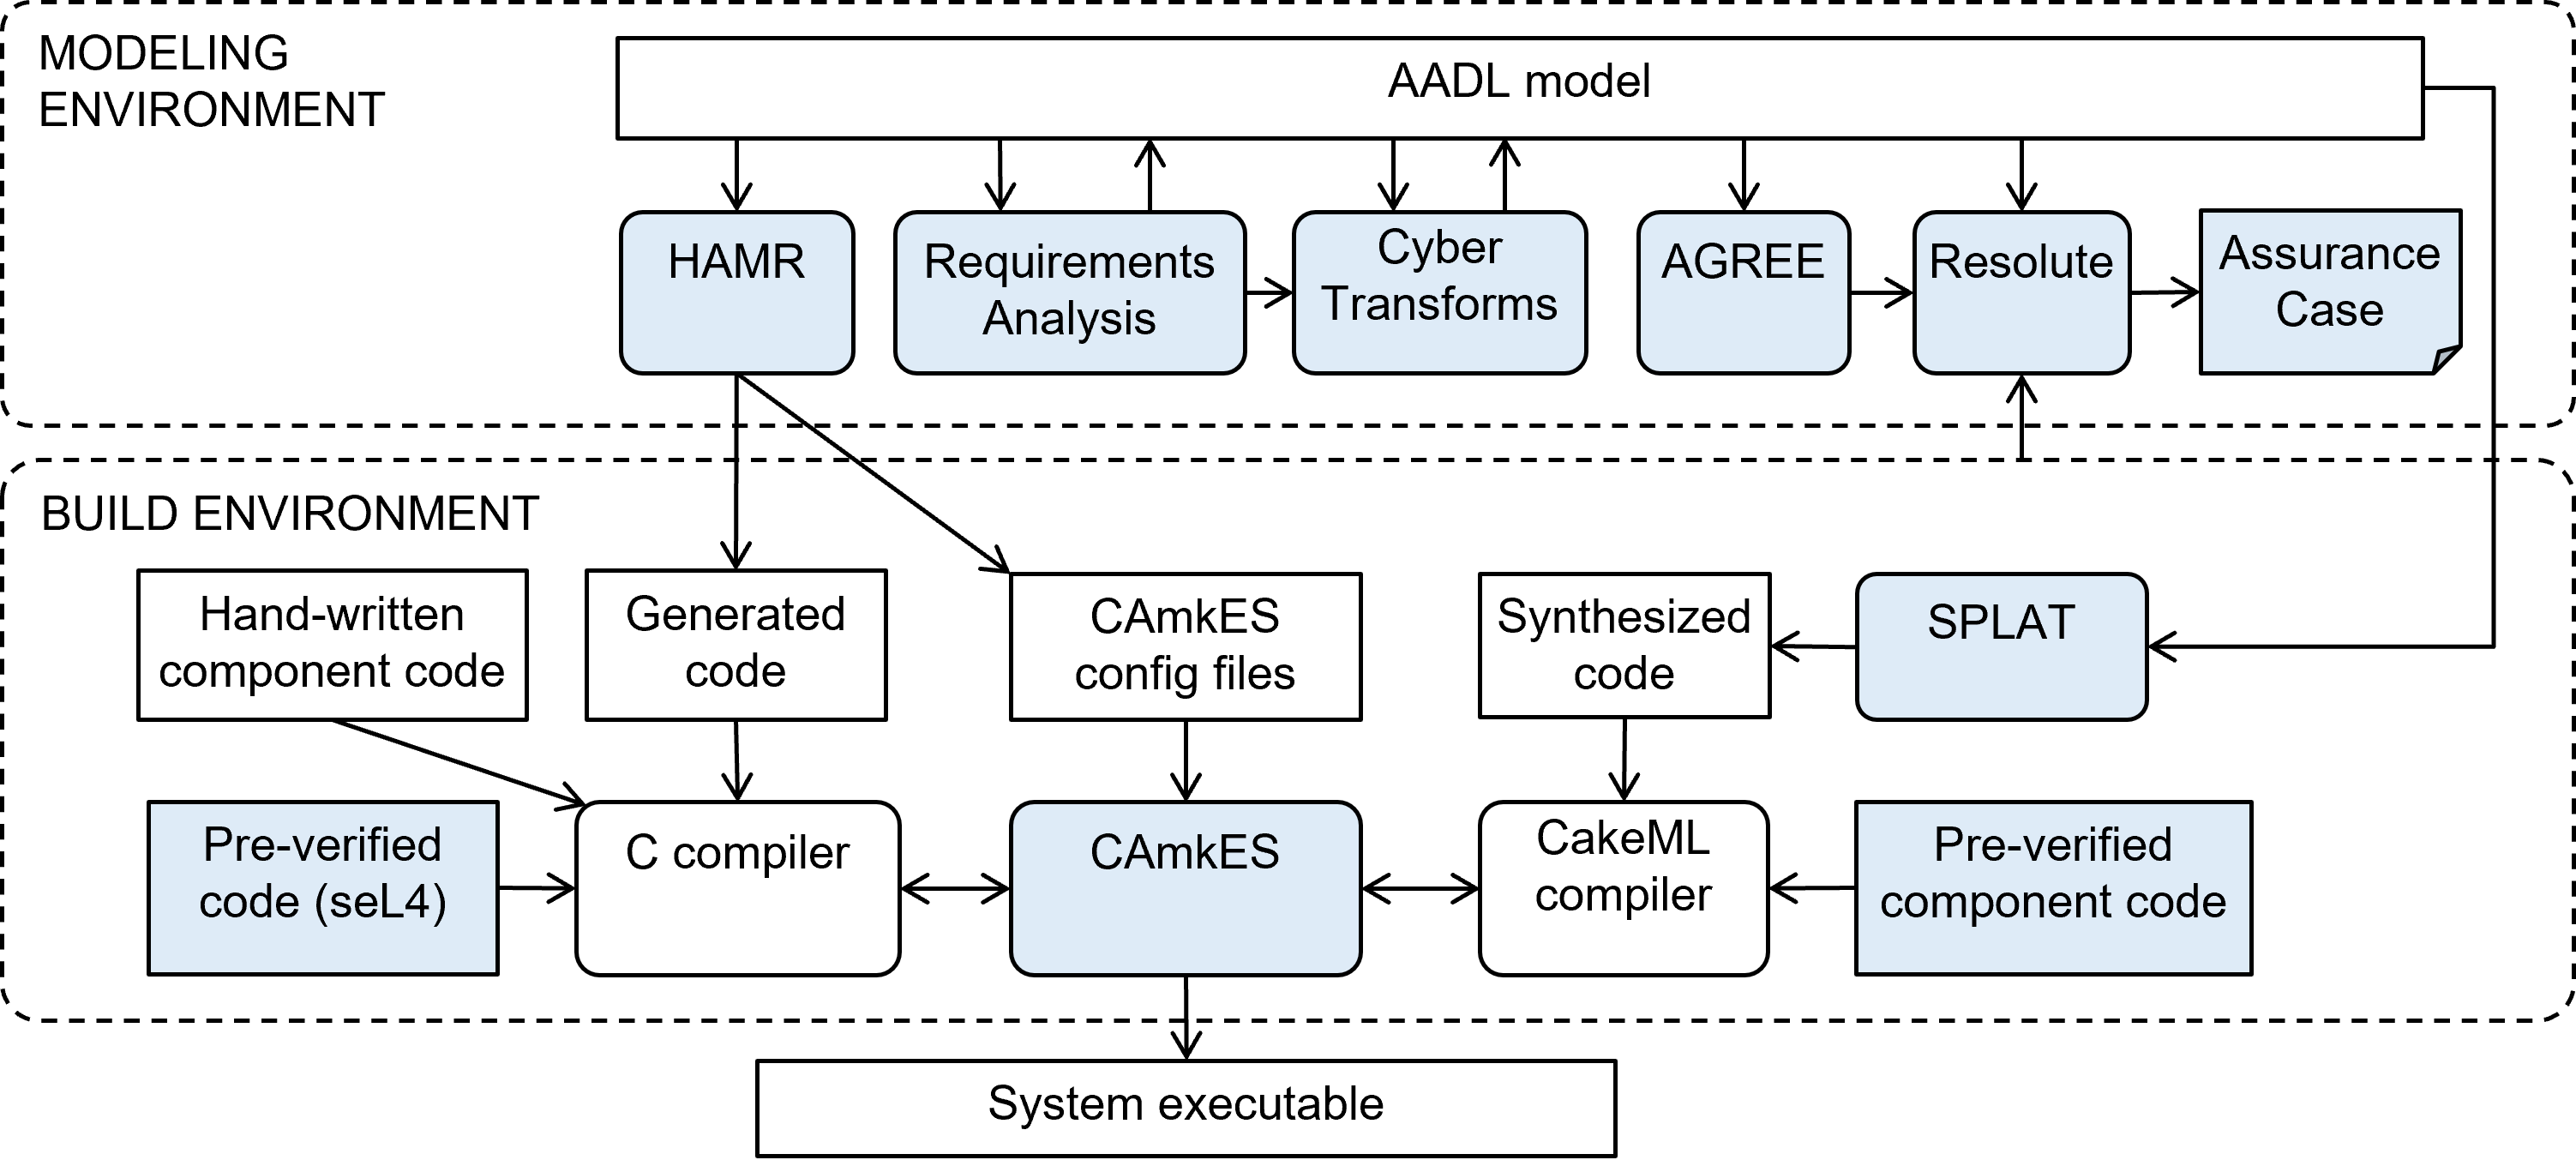
\includegraphics[width=\textwidth]{figs/briefcase-architecture.png}
	\caption{BriefCASE architecture. Tools and artifacts in the BriefCASE workflow are shown in blue.}
	\label{fig:briefcase-architecture} 
\end{figure}


%	Cyber analysis / Req generation
BriefCASE provides access to two architecture analysis tools (GearCASE~\cite{gearcase2020} and DCRYPPS~\cite{dcrypps2019}) that analyze AADL models for potential cyber vulnerabilities and generate cyber requirements for mitigation. 
Systems engineers are presented with a requirements management interface for viewing the generated requirements and importing them into the model so they can be addressed.  
Some requirements can also be formalized as assume-guarantee contracts added to the AADL model, enabling formal verification. Such a requirement will be imported into the model with with an associated formal contract.

%	Model transformation
To address a new cyber requirement, the architecture will need to be transformed in such a way as to harden the design against the vulnerability. BriefCASE provides an extendable library of model transformations for addressing common cyber vulnerabilities. 
The transformations are automated by the BriefCASE tool, resulting in a hardened model that is correct-by-construction. 
For example, the requirement that a component only receives well-formed messages can be satisfied by the insertion of a high-assurance filter. A BriefCASE transform wizard helps to configure the filter component properties, including the filter behavioral specification, which is represented as an assume-guarantee contract. BriefCASE then inserts a new filter component into the model, sets the component properties, and establishes the appropriate connections to source and destination components. The filter behavioral contract is also added to the model, enabling formal analysis of the model as well as providing the behavioral specification for a provably correct synthesis of the filter component implementation. 
The transformation also updates the assurance case with new evidential statements indicating how the associated goal has been satisfied, including the strategy used and links to context and associated evidence needed for assurance case evaluation.

%	Compositional analysis
The Assume Guarantee Reasoning Environment (AGREE)~\cite{compositional-analysis-agree}, is a compositional, assume-guarantee-style model checker for AADL models. AGREE attempts to prove properties about one layer of the architecture using properties allocated to subcomponents. The composition is performed in terms of assumptions and guarantees that are provided for each component.  
Once the system architecture has been modeled in AADL and component assume-guarantee contracts have been specified, the AGREE model checker is used to verify the consistency of these contracts.
%
%1) Component interfaces – The output guarantees of each component must be strong enough to satisfy the input assumptions of downstream components.
%
%2) Correctness of implementations – The input assumptions of a system along with the output guarantees of its sub-components must be strong enough to satisfy its output guarantees. 
% 
%This hierarchical strategy for reasoning about contracts, or compositional analysis, reduces the computational complexity of model checking by breaking down the larger problem into more manageable fragments.  
AGREE results are automatically incorporated as evidence into the BriefCASE assurance case.

%	High-Assurance Component synthesis
The correctness of the high-assurance components inserted by BriefCASE transformations means that each such component must meet its AGREE contract. This obligation is addressed by formal synthesis, using the Semantic Properties of Language and Automata Theory (SPLAT) tool~\cite{case-models-2021}. SPLAT generates code to implement the AGREE contract and then proves that its implementation exactly preserves the meaning of the contract all the way down to the binary for the target platform.

SPLAT uses the HOL4 theorem proving system to implement the synthesis and prove its correctness relative to the contract. The synthesis targets a dialect of Standard ML called CakeML and uses CakeML’s fully verified compiler to render the final binary~\cite{cakeml}. 
The SPLAT proof shows equivalence between the contract and the synthesized CakeML, leveraging the existing CakeML compiler proof, and reasons about the perpetual re-execution of the code as scheduled in a real-time environment.

%	Infrastructure Code Generation
BriefCASE employs the High Assurance Modeling and Rapid engineering for embedded systems (HAMR) tool~\cite{hamr}, a multi-platform, multi-language AADL code generation framework. 
Using seL4~\cite{sel4-sosp09} as a foundation, HAMR enables AADL to be used as a model-based development and systems engineering framework for seL4-based applications. 
%
The seL4 microkernel is a lightweight, fast, and secure operating system kernel. Its implementation is fully formally verified, from high-level security properties down to the binary level.
%
One of the primary objectives of HAMR is to support system builds that leverage seL4 separation and information flow guarantees to achieve the AADL-specified component isolation and inter-component communication needed for cyber-resiliency. 

For each AADL thread component, HAMR generates a thread code skeleton and APIs for communicating over the ports declared on the component. For components that are implemented manually, the developer fills out the thread skeleton with application code. 
%
HAMR generates component infrastructure and integration code implementing the semantics of AADL-compliant thread scheduling, thread dispatching, and port-based communication. 

The seL4 deployment uses the Component Architecture for microkernel-based Embedded Systems (CAmkES) code-generation framework to configure the microkernel. The HAMR-generated CAmkES directly encodes the AADL model’s component and communication topology and includes the AADL run-time infrastructure with its thread scheduling. HAMR leverages the existing seL4 domain scheduler to enforce time partitioning and provide static cyclic scheduling. 
%
As part of its code generation process, HAMR produces flow graphs reflecting the inter-component information flow at both the AADL architecture level and the CAmkES level for the seL4 deployment. Visual representations are provided for manual inspection, and SMT-based representations are generated for formal reasoning. The SMT-based representations are used to prove that 1) all AADL modeled flows are in the CAmkES configuration, and 2) no extraneous flows have been added. 


\subsection{Assurance Case Generation in BriefCASE}

% Resolute
Each of the BriefCASE tools contribute to an aspect of high-assurance systems development, and each emit evidence of correctness that can be used to substantiate cyber-resiliency assurance goals. Resolute~\cite{resolute2014} is used to evaluate this evidence and incorporate it into a system cyber-resiliency assurance case. 
%
%	Very high-level overview of Resolute
Resolute is a language and tool for embedding an assurance argument in an AADL system architecture model and evaluating the validity of the associated evidence.

%	Maintaining cyber requirements in Resolute
A BriefCASE project contains a repository for cyber requirements. Imported requirements (e.g., those generated by GearCASE or DCRYPPS) are represented as assurance case goals to be satisfied. 
For example, a requirement that specifies that a target component shall only receive well-formed messages is imported as the Resolute \texttt{goal} depicted in Fig.~\ref{fig:resolute-requirement}a.  The goal is initially marked \texttt{undeveloped}.

\begin{figure}[h] 
	\centering 
	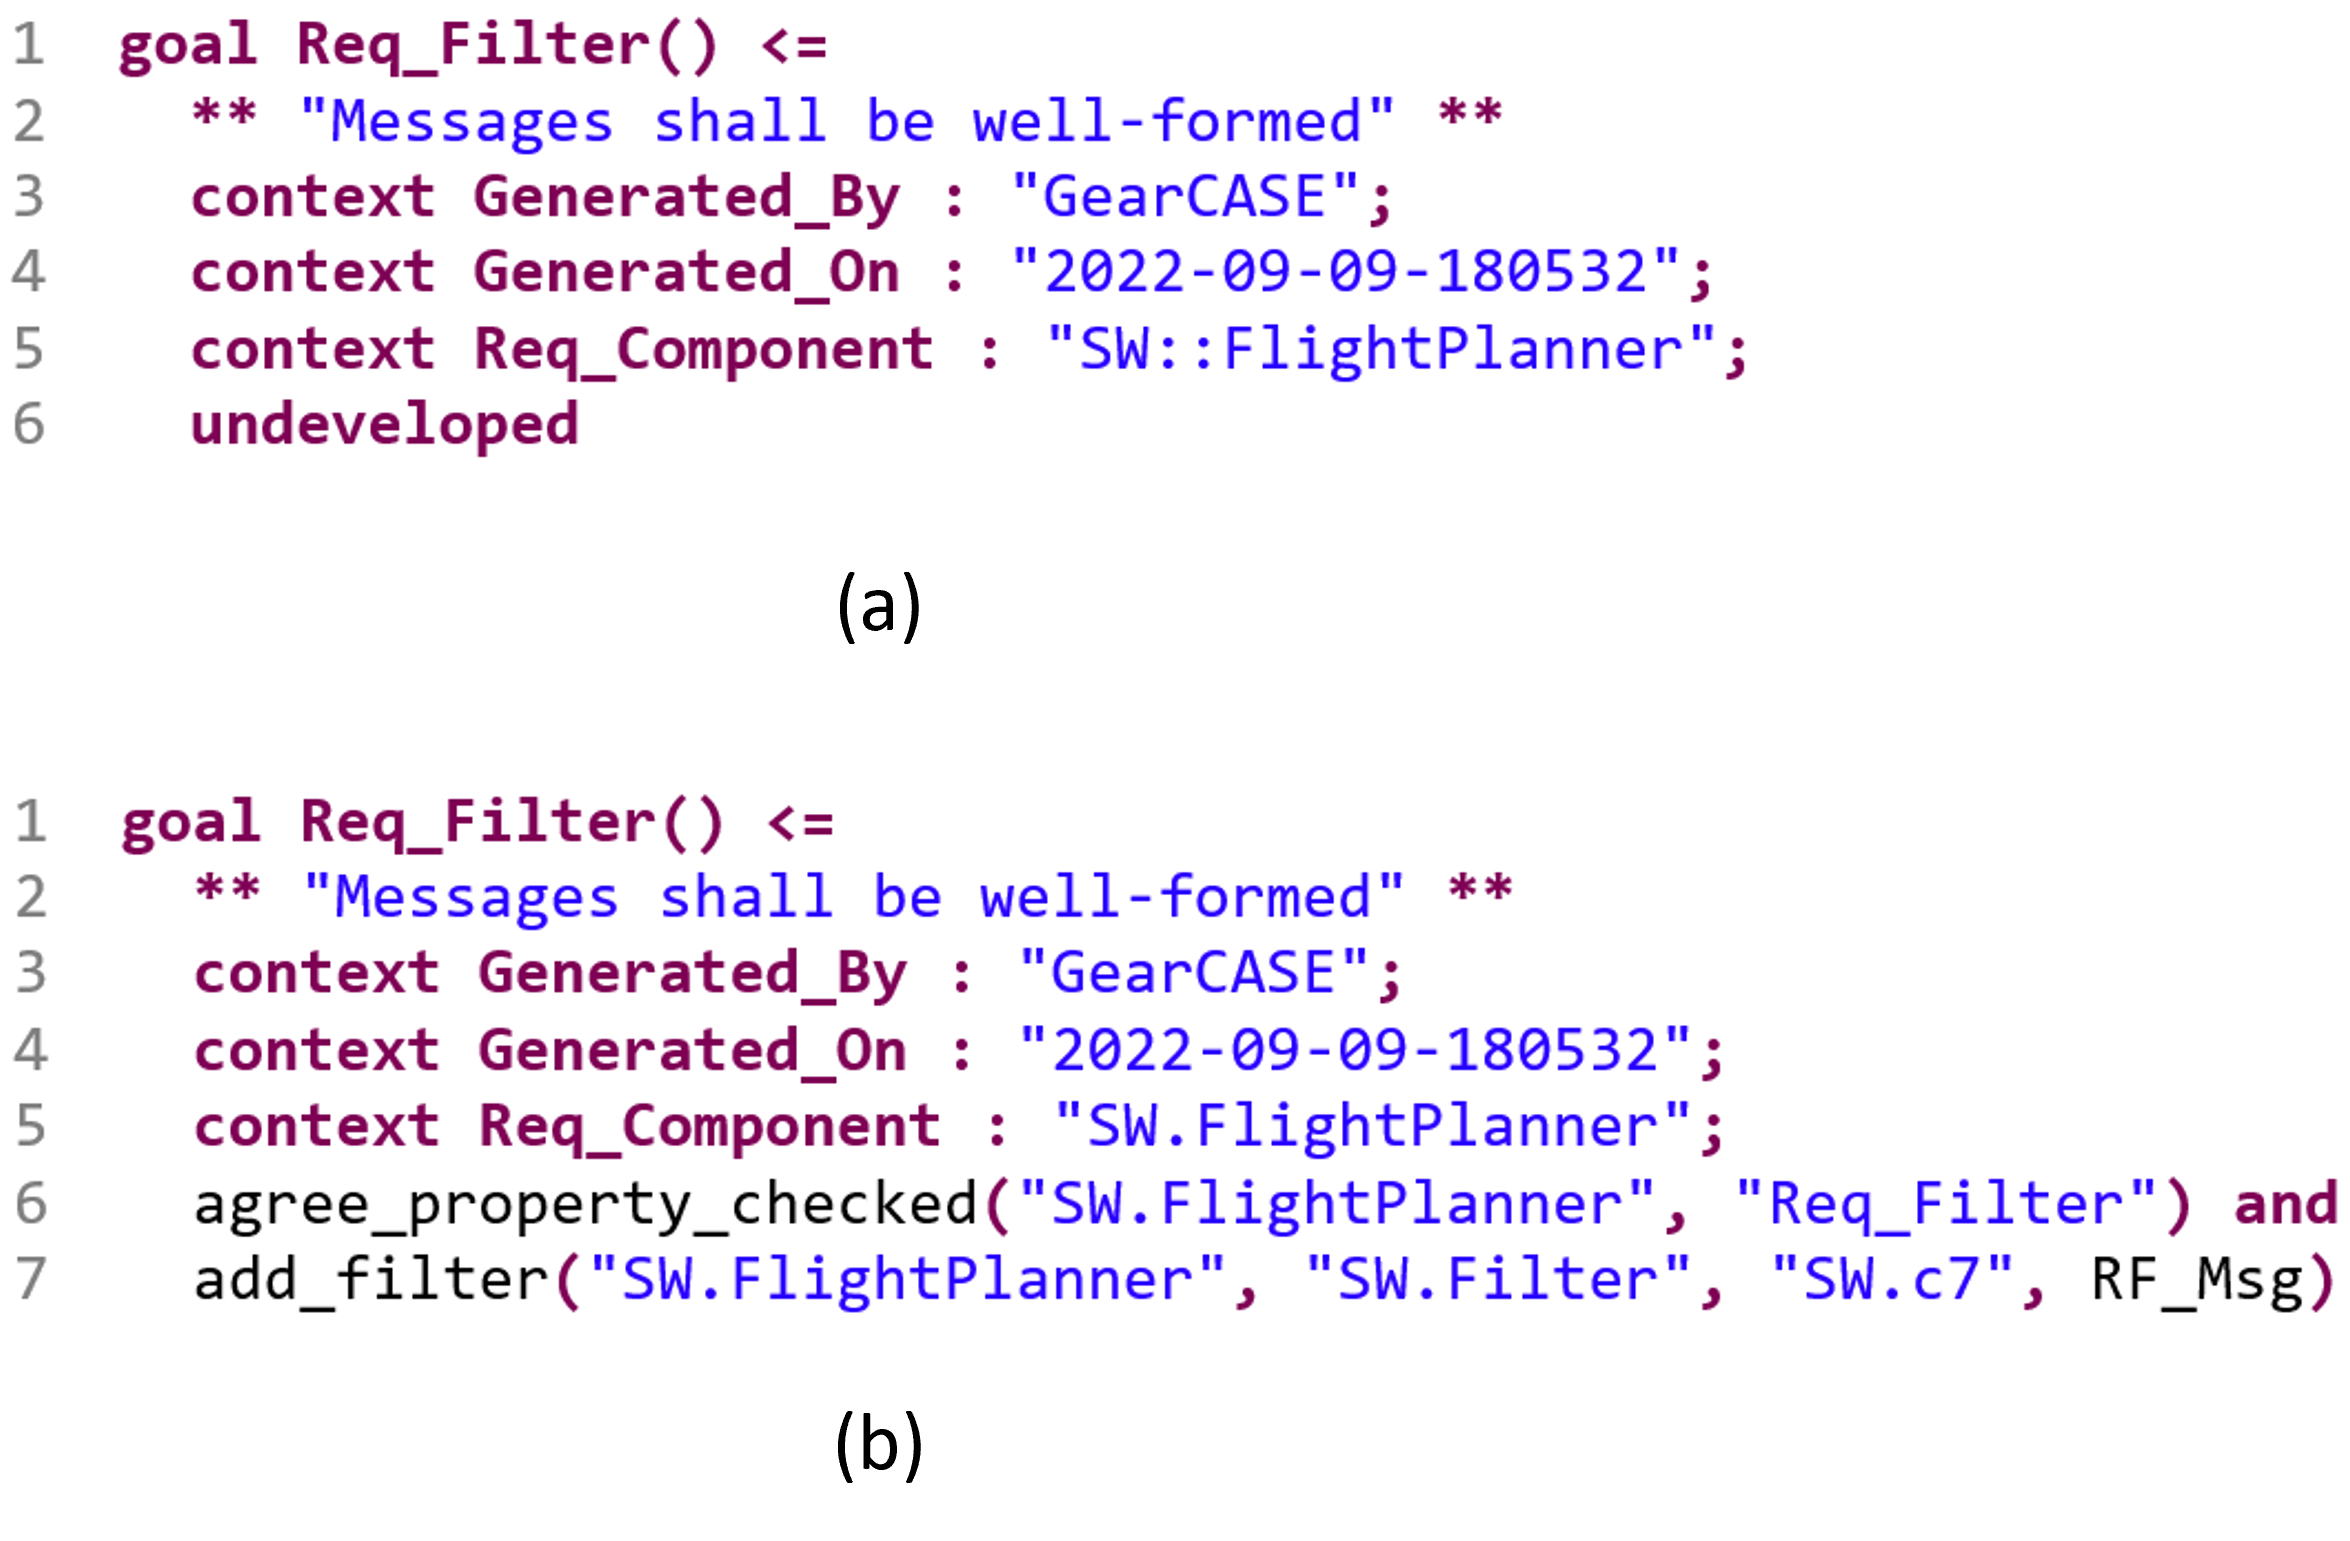
\includegraphics[width=\textwidth]{figs/resolute-requirement.png}
	\caption{(a) Cyber requirement imported as \textit{undeveloped} Resolute assurance goal.  (b) Updated goal with logical rules for determining whether goal is satisfied.}
	\label{fig:resolute-requirement} 
\end{figure}

%	Updating requirements with automated transform assurance library in BriefCASE
The well-formed message requirement can be mitigated by performing an automated model transformation for inserting a filter. Each transformation has an associated assurance pattern that describes a strategy for determining from the model whether the requirement has been satisfied (see Section~\ref{sec:requirements-satisfied-in-model}).  
These evidential statements are added to the goal as the design is updated to address the requirement, as shown in Figure~\ref{fig:resolute-requirement}b.  For the insertion of a filter, Resolute must now check that AGREE formal analysis passes (line 6) and the filter was added correctly to the model (line 7).  The \texttt{agree\_property\_checked()} and \texttt{add\_filter()} function definitions are included with the built-in BriefCASE assurance pattern library and contain additional statements that instruct Resolute on how to determine the validity of the claims. 
Subsequent changes to the model that invalidate any of the assurance claims can then be detected and corrected.  

%	Specifying external evidence in Resolute
Resolute has recently been updated to enable evaluation of artifacts external to the modeling workspace. An Artifact Management tool is included with BriefCASE for specifying how Resolute should parse documents with specific formats (such as test results, review forms, etc.) to determine whether they support specific assurance claims.  For each type of document, users can specify a regular expression that gets matched against the contents of the document, such that a correct match indicates the validity of the evidence in supporting a specific claim.

%	BriefCASE assurance pattern in Resolute
The assurance patterns presented in our previous work (see~\cite{resolute-destion}) primarily focused on design assurance; that is, correctness of the architecture model.  With recent updates to BriefCASE and Resolute, we have since expanded the pattern into a comprehensive cyber-resiliency assurance argument covering architecture design, code generation, and system build.  The assurance pattern is formalized in Resolute and included with BriefCASE.
%
We describe the BriefCASE system cyber-resiliency assurance pattern in the next section.


% Start high-level, go as low-level as space allows
% Don't go into too much detail of model argument, instead refer to Destion paper
% Spend more time on implementation argument?
\section{BriefCASE Cyber-Resiliency Assurance Pattern}
\label{sec:assurance-pattern}
% Overview of assurance argument structure
The high-level structure of our CASE assurance pattern is inspired by the D-MILS argument pattern~\cite{dmils}, in which system dependability properties are assured via modules arguing component, compositional, and implementation correctness.  
Although verifying functional, safety, and other dependability properties is necessary for a comprehensive system assurance case, the CASE pattern presented here only addresses cyber-resiliency.  The intention is for the resulting assurance argument to be integrated into a full system assurance case, when necessary.

The high-level CASE argument structure is depicted in Figure~\ref{fig:top-level}, with the top-level goal being ``The system is acceptably cyber-resilient".  
This goal is then substantiated by arguments that cyber-resiliency requirements have been appropriately identified and then satisfied, both in the system model and the \textit{realization} of the system model as a built, deployable system.

\begin{figure}[h] 
	\centering 
	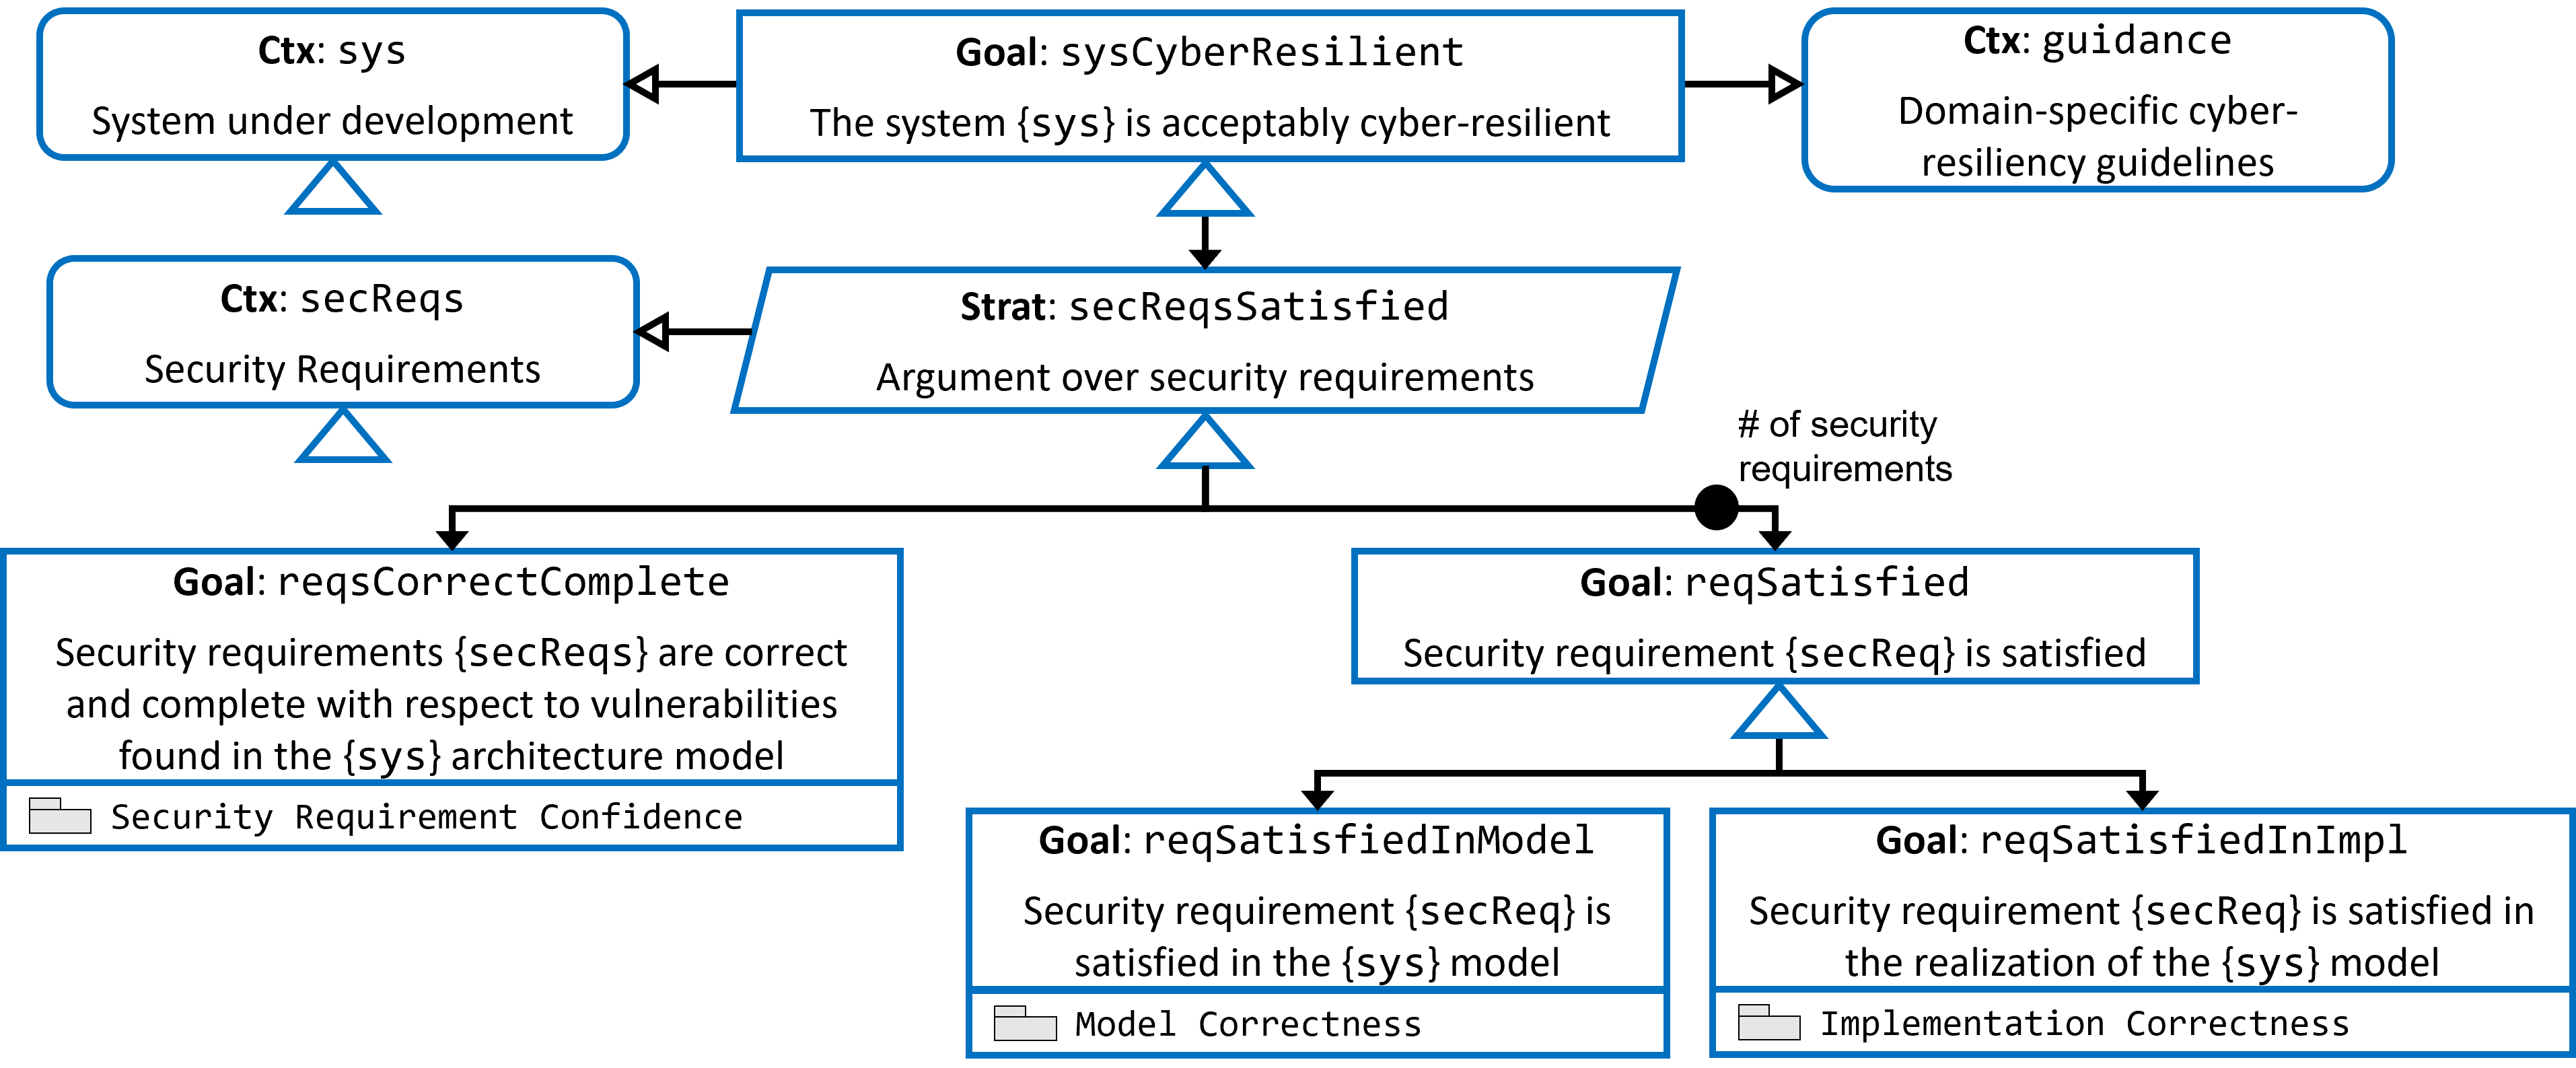
\includegraphics[width=\textwidth]{figs/top-level.png}
	\caption{Top-level assurance pattern structure.}
	\label{fig:top-level} 
\end{figure}


% Describe at a high-level how each workflow step should be assured.  Refer to figure.  Then dive into BriefCASE assurance pattern.

% Security requirements are correct and complete
\subsection{Cyber Requirement Correctness and Completeness}
BriefCASE currently includes two cybersecurity plug-ins, GearCASE~\cite{gearcase2020} and DCRYPPS~\cite{dcrypps2019}, that analyze an AADL model and output a set of cyber requirements corresponding to vulnerabilities detected in the model.  
BriefCASE maintains the generated requirements within the framework as assurance goals using the Resolute tool~\cite{resolute2014}.  
In addition to providing an AADL annex grammar for representing assurance cases, Resolute includes an evaluation engine for determining whether sufficient evidence exists (both internal and external to the AADL workspace) to support assurance claims.  
Because BriefCASE manages the development artifacts associated with the CASE workflow, it automatically provides Resolute with instructions on how those artifacts can be used to support specific cyber-resiliency goals.
%Resolute generates assurance arguments in a tree format, but also supports export to graphical tools such as AdvoCATE~\cite{advocate}.  


The assurance argument for cybersecurity requirement correctness and completeness is shown in Figure~\ref{fig:req-correct-complete}.  
%
In the figure, it can be seen that in order to support the claim, we must provide evidence that the full set of cyber requirements passed through a review process, were imported into the BriefCASE environment as Resolute goals or omitted with rationale, and that successive analyses on updated versions of the model finds no new vulnerabilities.  The latter reflects the iterative step in the workflow (depicted by the left-pointing arrow in Figure~\ref{fig:workflow}), in which a modified model must be re-analyzed after applying a mitigation for a previously generated requirement.  This is necessary in order to demonstrate that the mitigation of one vulnerability does not inadvertently introduce other vulnerabilities.  To argue that the current model was analyzed appropriately, we must be able to demonstrate that the model is well-formed; that is, it complies with modeling guidelines, that the analysis was indeed performed on the current version of the model, and that the analysis does not produce any new applicable requirements.

\begin{figure}[h] 
	\centering 
	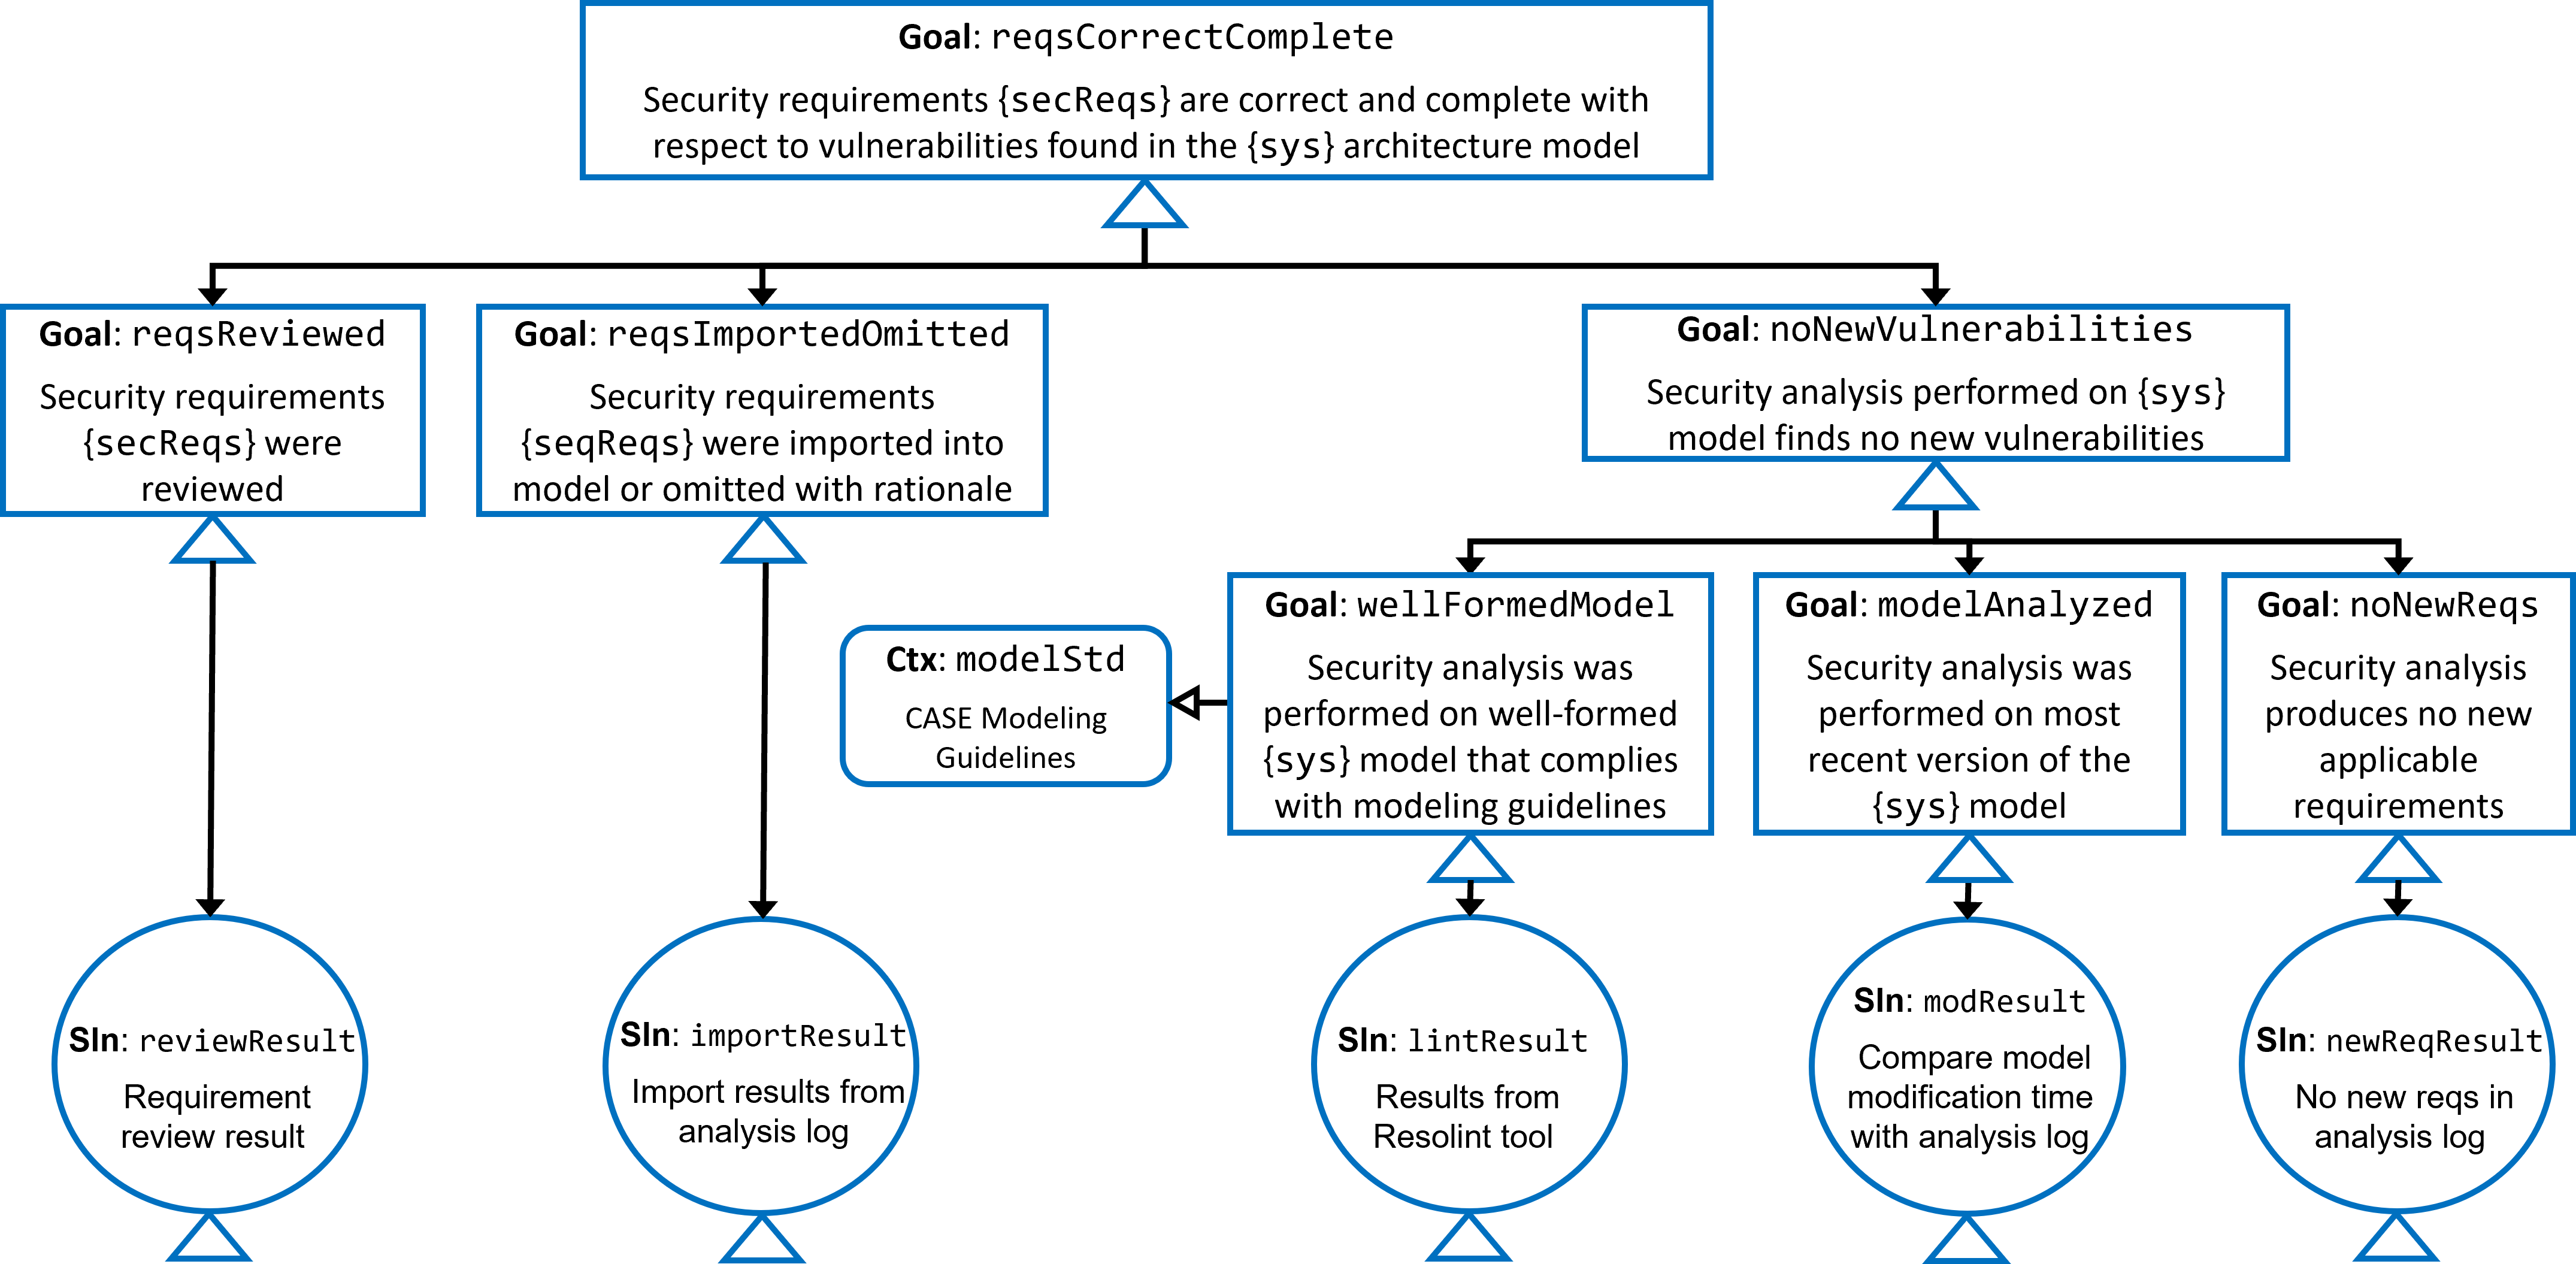
\includegraphics[width=\textwidth]{figs/req-correct-complete.png}
	\caption{Assurance pattern for security requirement correctness and completeness.}
	\label{fig:req-correct-complete} 
\end{figure}

% Model assurance
\subsection{Cyber Requirements are Satisfied in the System Model}
BriefCASE includes a library of automated model transformations corresponding to common cyber requirement classes.  Each transformation modifies the model to harden it against a specific vulnerability, thereby mitigating the associated threat and addressing the driving requirement.  In addition, the transformations automatically update the corresponding Resolute goals with instructions that enable Resolute to evaluate whether the goal is supported by the necessary evidence.

% NOT SURE HOW MUCH SPACE WE WILL HAVE HERE.
% USE FILTER AS EXAMPLE
% OTHERWISE, JUST REFERENCE DESTION PAPER 
Because the transformations modify the architecture model in different ways, assuring that a specific requirement is satisfied in the model will be argued according to a transformation-specific pattern.  For example, a well-formed message requirement on a component's input port can be addressed by inserting a filter on the communication channel upstream of the target component.  The corresponding assurance pattern for this mitigation is shown in Figure~\ref{fig:filter}.  Here, we argue that the well-formed message requirement has been satisfied in the model by showing that formal verification passed on the current version of the model, that a filter is appropriately inserted upstream of the target component, and that the filter cannot be bypassed.  Assurance patterns corresponding to all the BriefCASE model transformations have been defined and are packaged with the tool.  Due to space limitations we do not include them here, but instead refer the reader to the BriefCASE User's Guide~\cite{BriefCASE-user-guide}.

\begin{figure}[h] 
	\centering 
	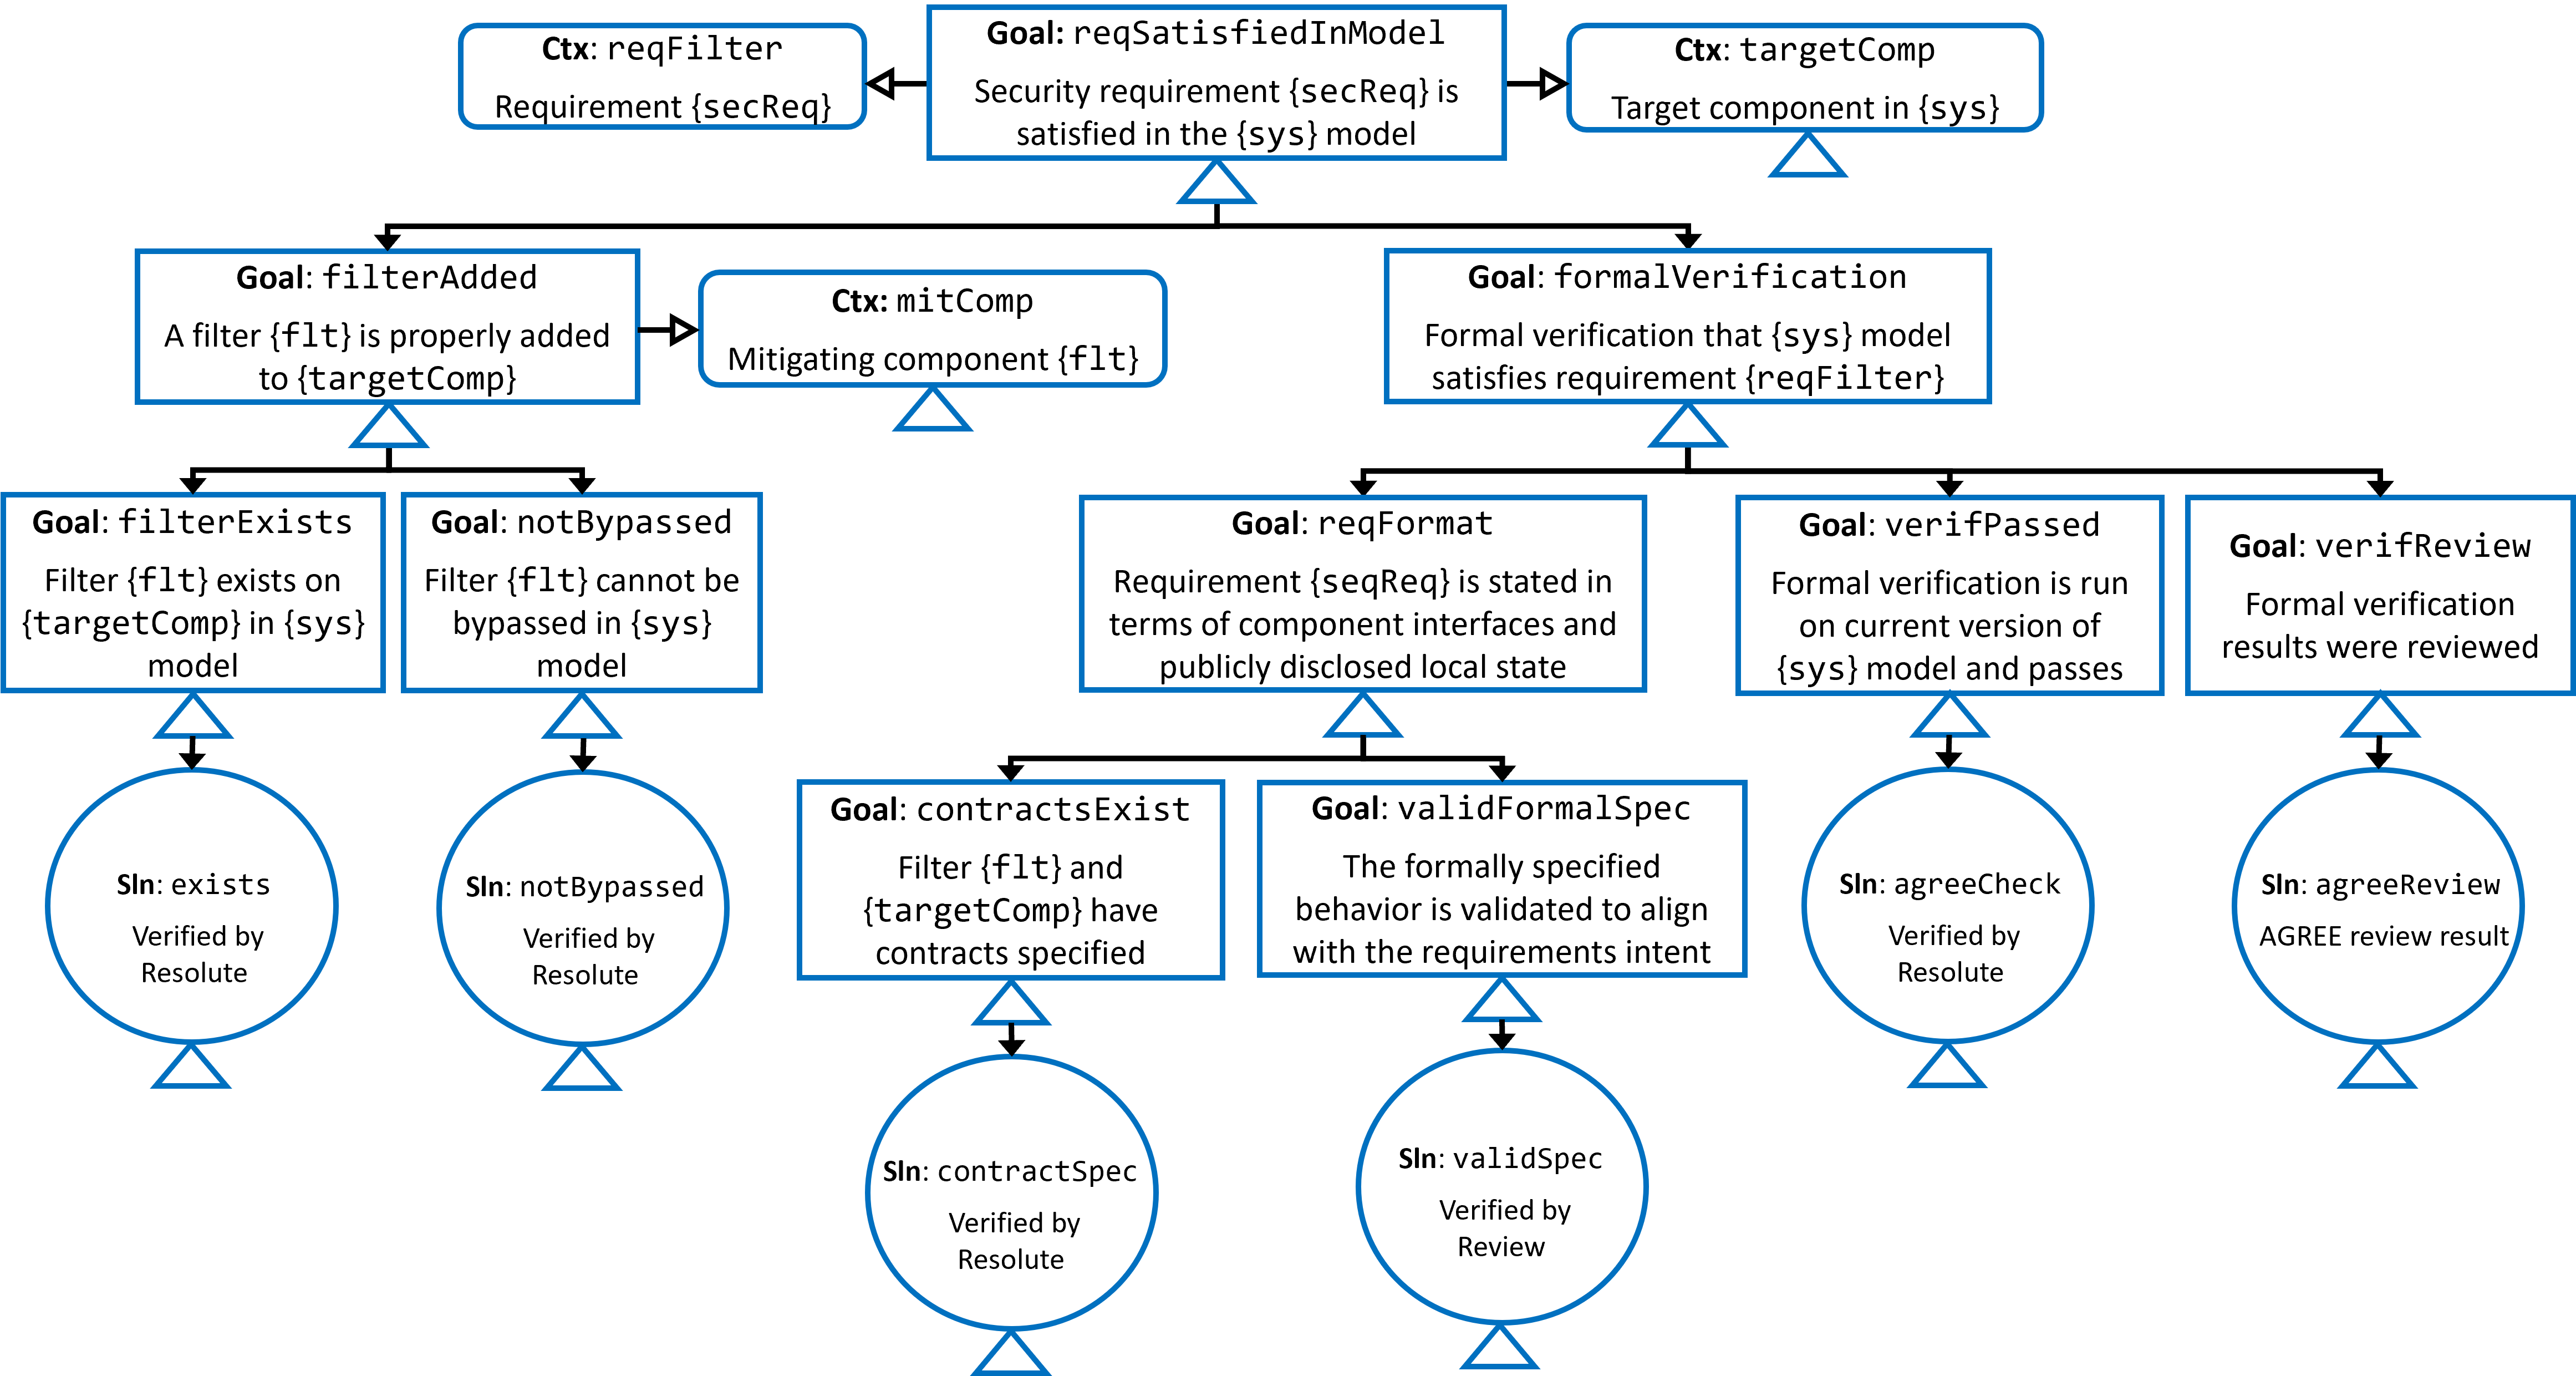
\includegraphics[width=\textwidth]{figs/filter.png}
	\caption{Pattern for assuring proper filter mitigation in the architecture model.}
	\label{fig:filter} 
\end{figure}

% Implementation assurance
\subsection{Cyber Requirements are Satisfied in the Realization of the System Model}
% Where BriefCASE implementations can come from (legacy/manual implementation, SPLAT synthesis, pre-packaged - Attestation, seL4, HAMR)

In the CASE workflow, a software component implementation could have various origins.  It could be legacy, third-party, or manually implemented code. It could also be generated from a behavioral model such as Simulink or be synthesized directly from the component's contract.  In BriefCASE, the latter is performed by the SPLAT tool~\cite{case-verified-filter}, which synthesizes the implementation of high-assurance components in the CakeML language~\cite{cakeml} directly from a formal assume-guarantee contract specified in the AADL component's AGREE annex~\cite{compositional-analysis-agree}.  In addition to providing a formally verified compiler, CakeML enables SPLAT to generate a proof that the synthesized implementation is correct with respect to the formal contract.

Application infrastructure code and the operating system itself must also be implemented and integrated into a deployable system.  BriefCASE employs the HAMR build tool~\cite{hamr}, which generates the infrastructure code, along with correspondence proofs that the inter-component connections specified in the model are maintained in the implementation and that no new connections have been created.  For high-assurance systems, this is made possible in part by building to a target platform running seL4~\cite{sel4-cacm18}, a formally verified microkernel that provides time and space partitioning guarantees.

% Add a paragraph (and maybe a figure?) on the HAMR API for component code to tie into following sentence
\todo{Brief description of HAMR API?}

\begin{figure}[h] 
	\centering 
	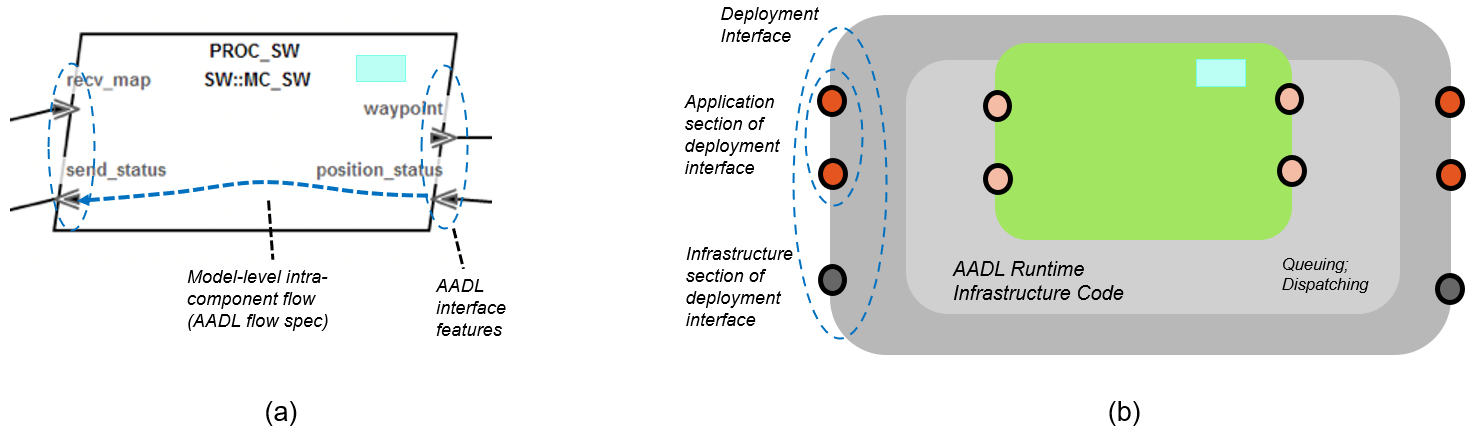
\includegraphics[width=\textwidth]{figs/deployment-interface.png}
	\caption{(a) Example AADL component interface features and disclosed component state. (b) Schematic of deployed component, with notion of observation points.}
	\label{fig:deployment-interface} 
\end{figure}

The structure of the \textit{model realization} branch of the assurance pattern (partially shown in Figure~\ref{fig:req-satisfied-in-model-realization}) therefore necessarily focuses on evidence of correctness in terms of behaviors observed at deployment observation points associated with the BriefCASE workflow.  
%Patterns for assuring deployed code with provenance external to BriefCASE are not presented here, but would be included in a straight-forward manner.


\begin{figure}[h] 
	\centering 
	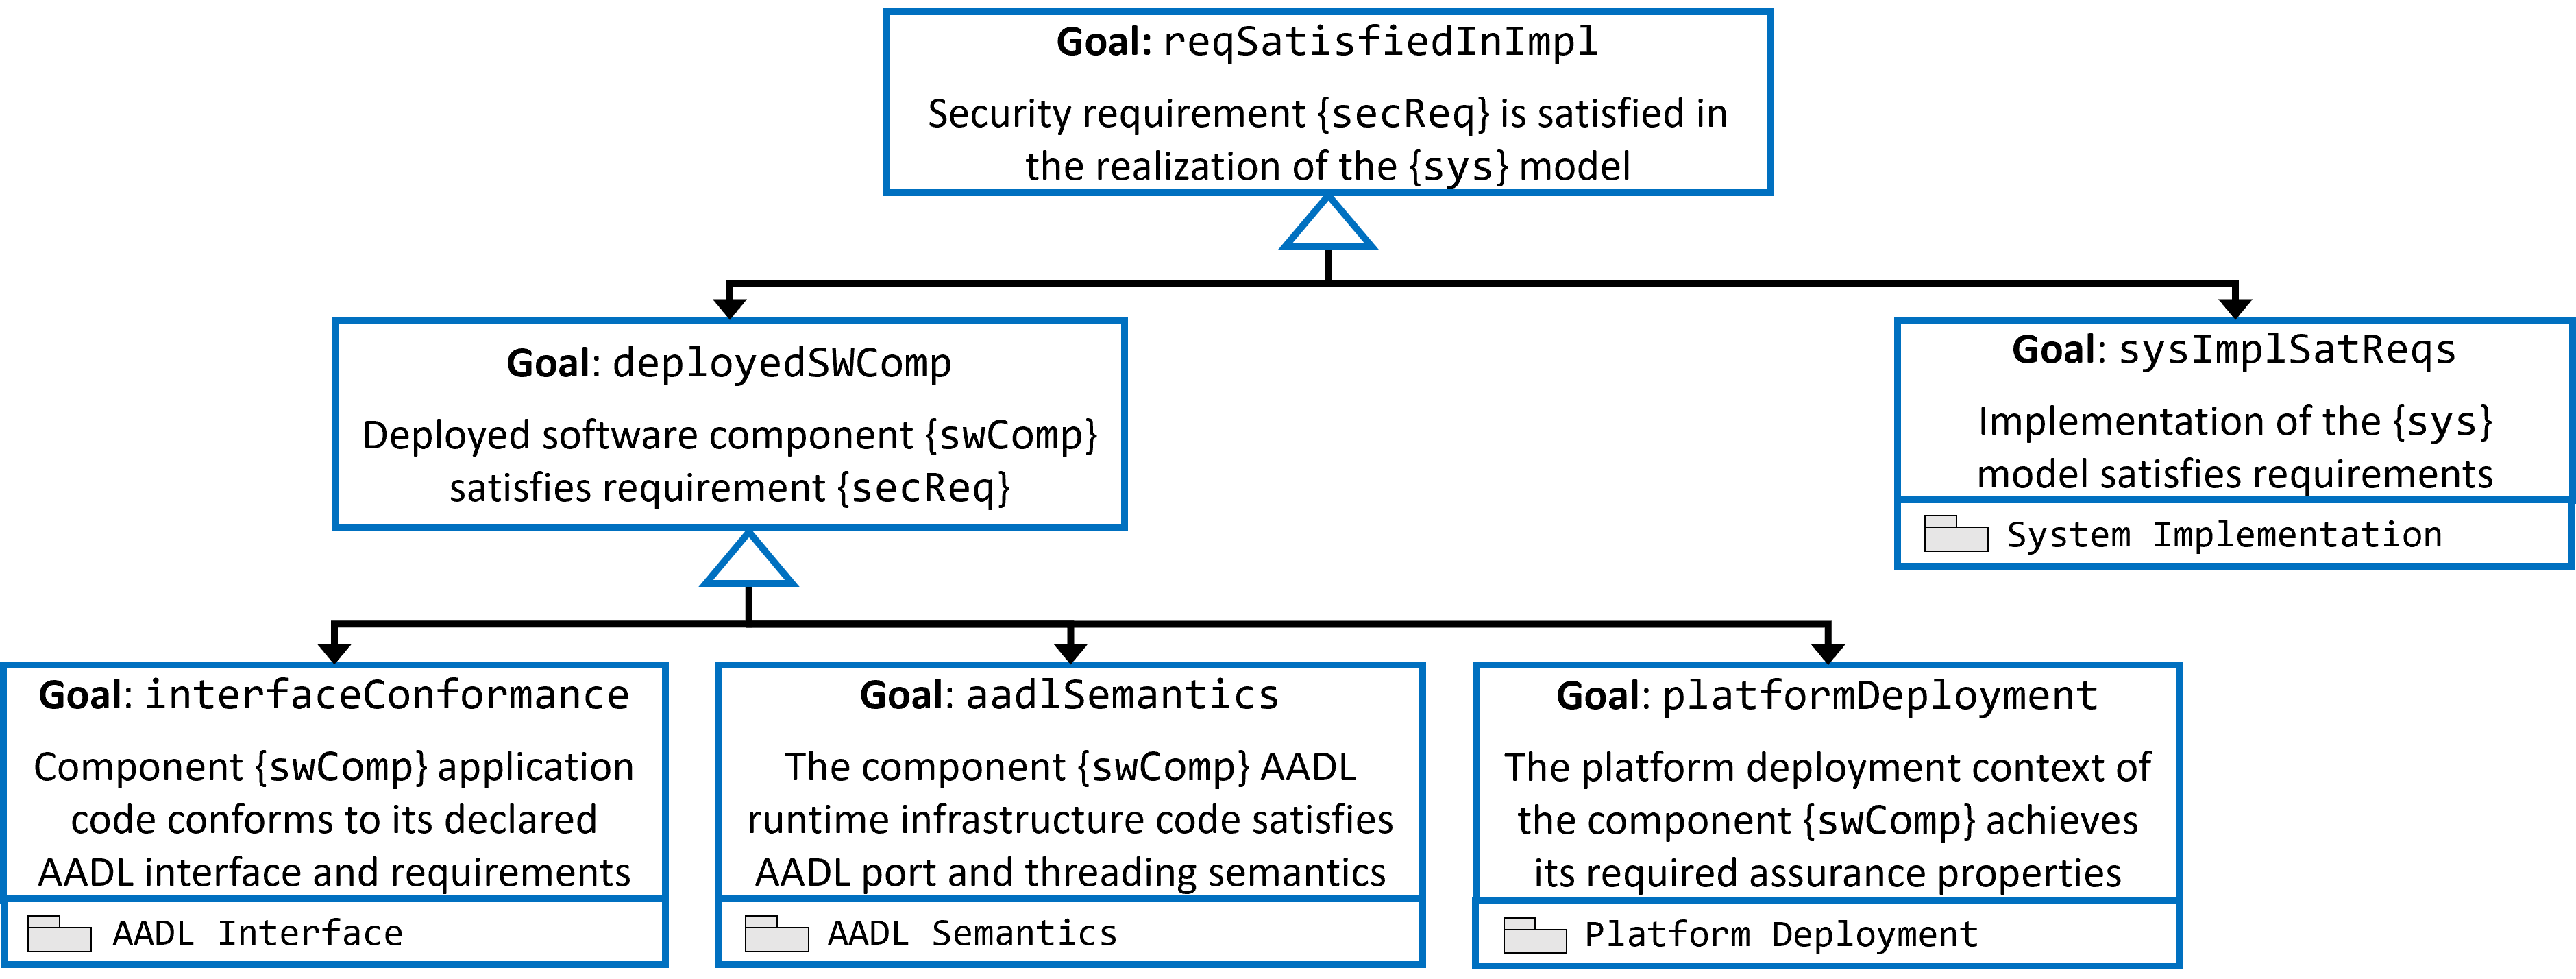
\includegraphics[width=\textwidth]{figs/req-satisfied-in-model-realization.png}
	\caption{Assurance pattern for arguing the requirement is satisfied in the realization of the model.}
	\label{fig:req-satisfied-in-model-realization} 
\end{figure}

To support the claim that the deployed software components satisfy their requirements,
%in Figure~\ref{fig:req-satisfied-in-model-realization}
for each component, we require evidence that the cyber requirements are stated in terms of a component's AADL interface and publicly disclosed state, and that the component application code conforms to both its declared interface and requirements.  Although demonstrating that requirements are stated in terms of a component's interface is not strictly necessary in the general case, it is included in this pattern for confidence that the CASE workflow was followed correctly. 


Furthermore, the component's application code must conform to its declared interface and requirements.  This goal is substantiated by the argument in Figure~\ref{fig:code-conforms-to-interface-and-requirements}.
%
% The component's AADL runtime infrastructure code satisfies AADL port and threading semantics
%
Finally, the component's platform deployment context achieves its required assurance properties.  This is supported by the argument in Figure~\ref{fig:platform-deployment-context-achieves-assurance-properties}.


\begin{figure}[h]
	\centering 
	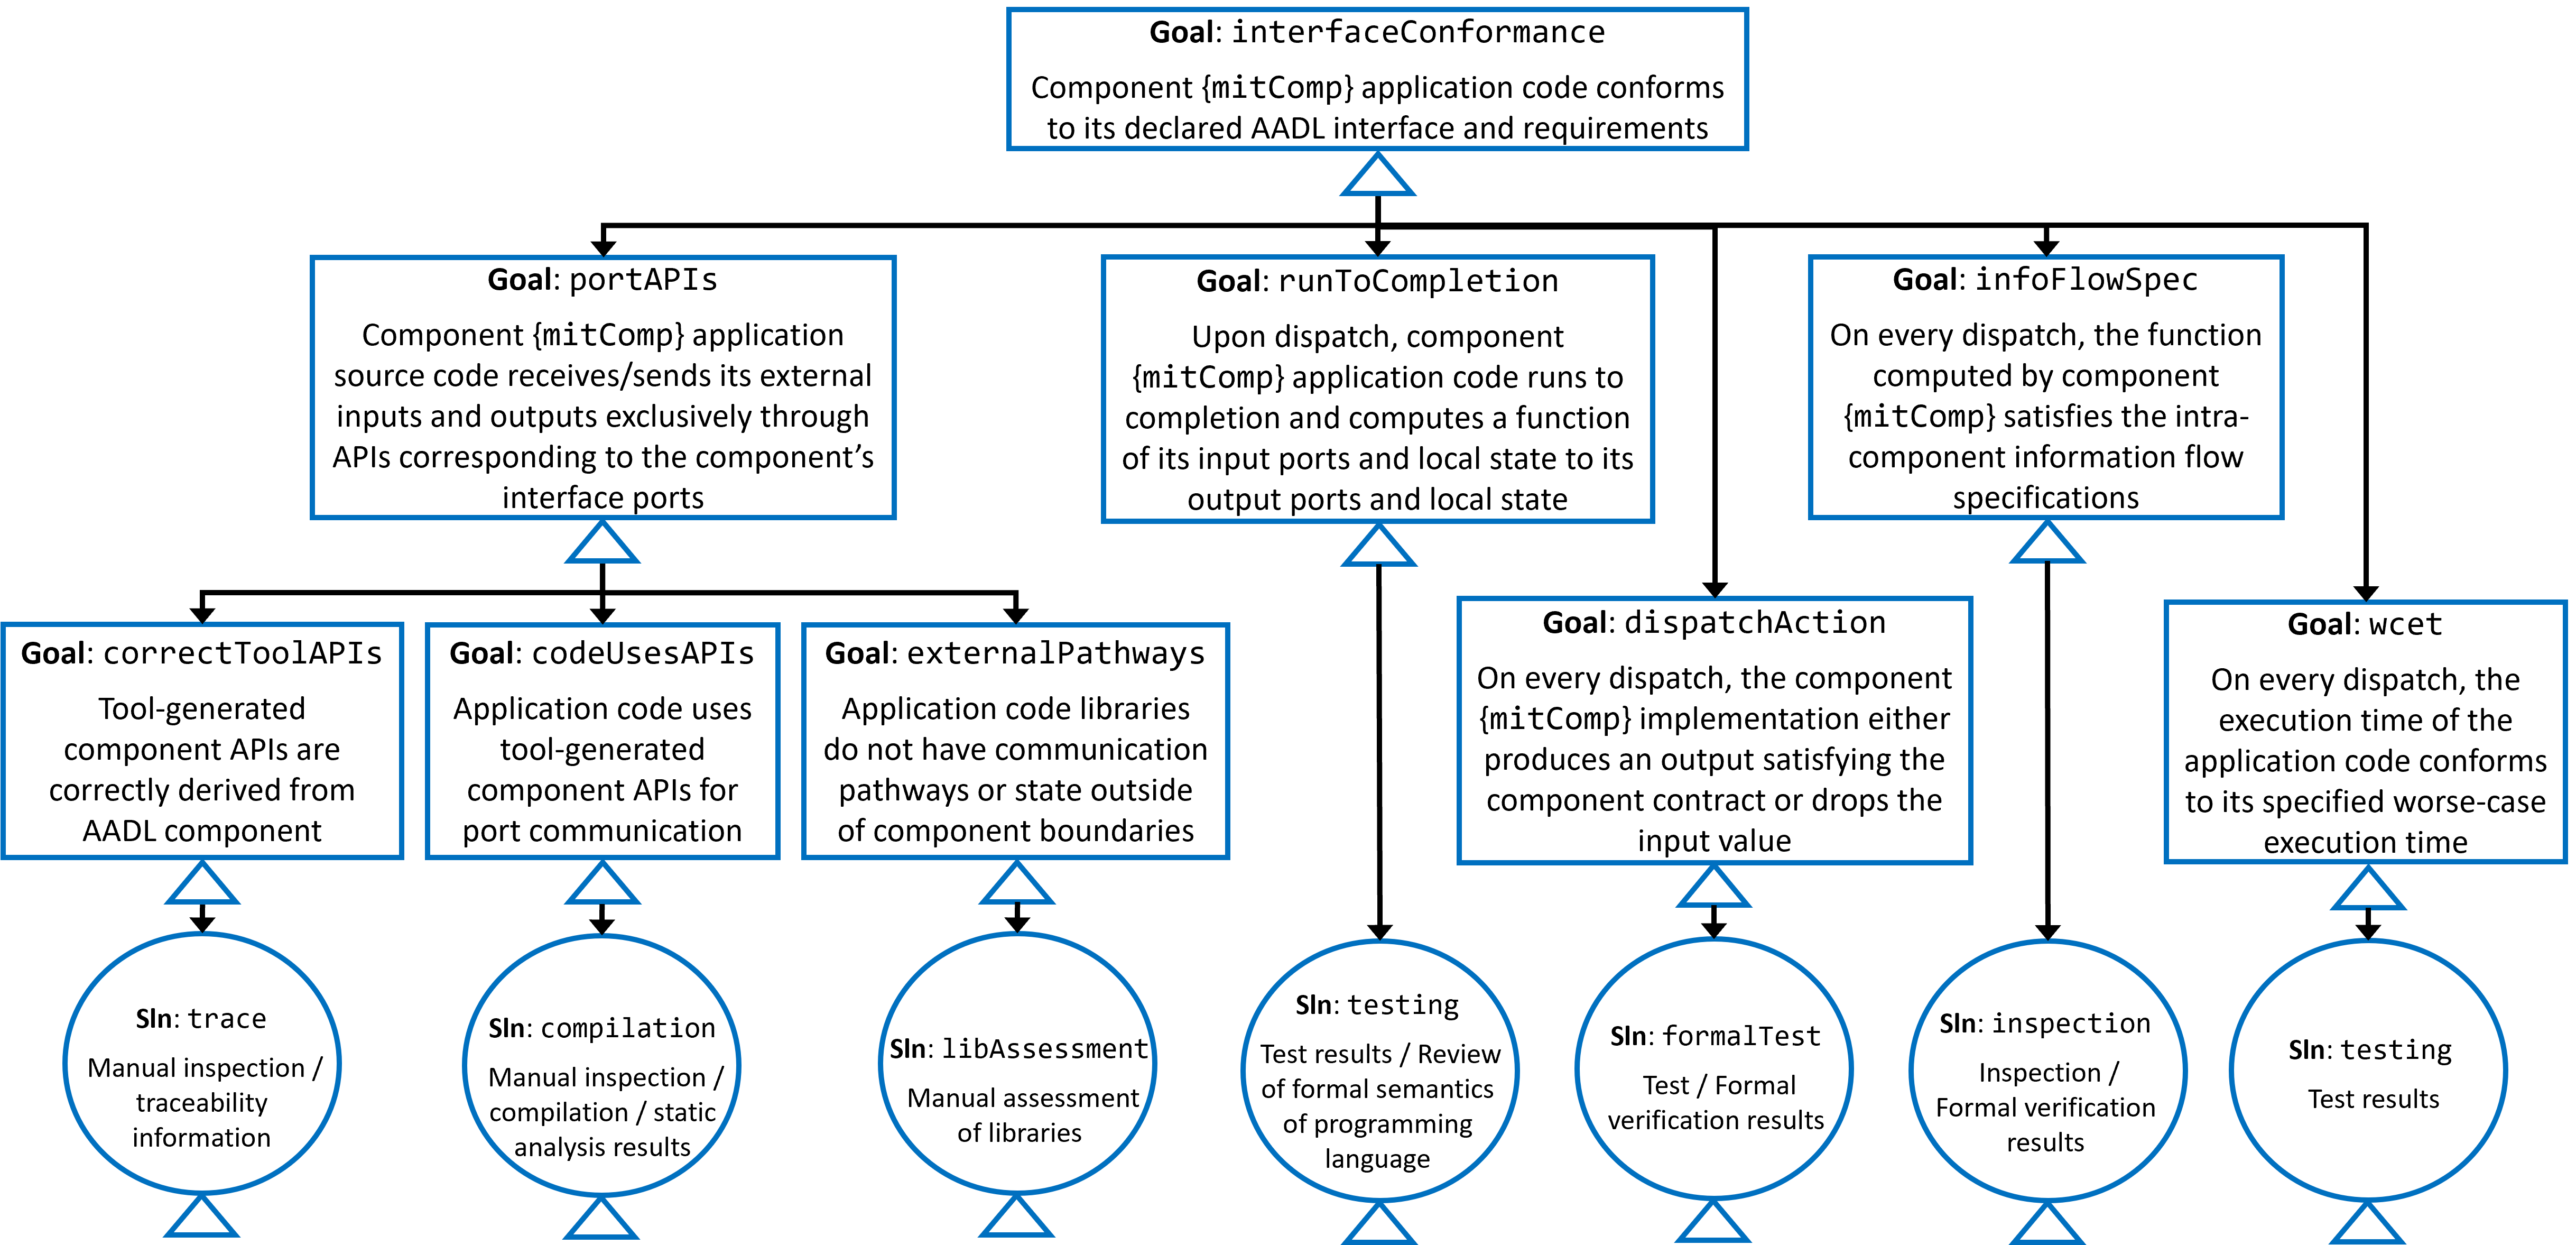
\includegraphics[width=\textwidth]{figs/code-conforms-to-interface-and-requirements.png}
	\caption{Assurance pattern for arguing component code conforms to the specified interface and requirements.}
	\label{fig:code-conforms-to-interface-and-requirements} 
\end{figure}


\begin{figure}[h] 
	\centering 
	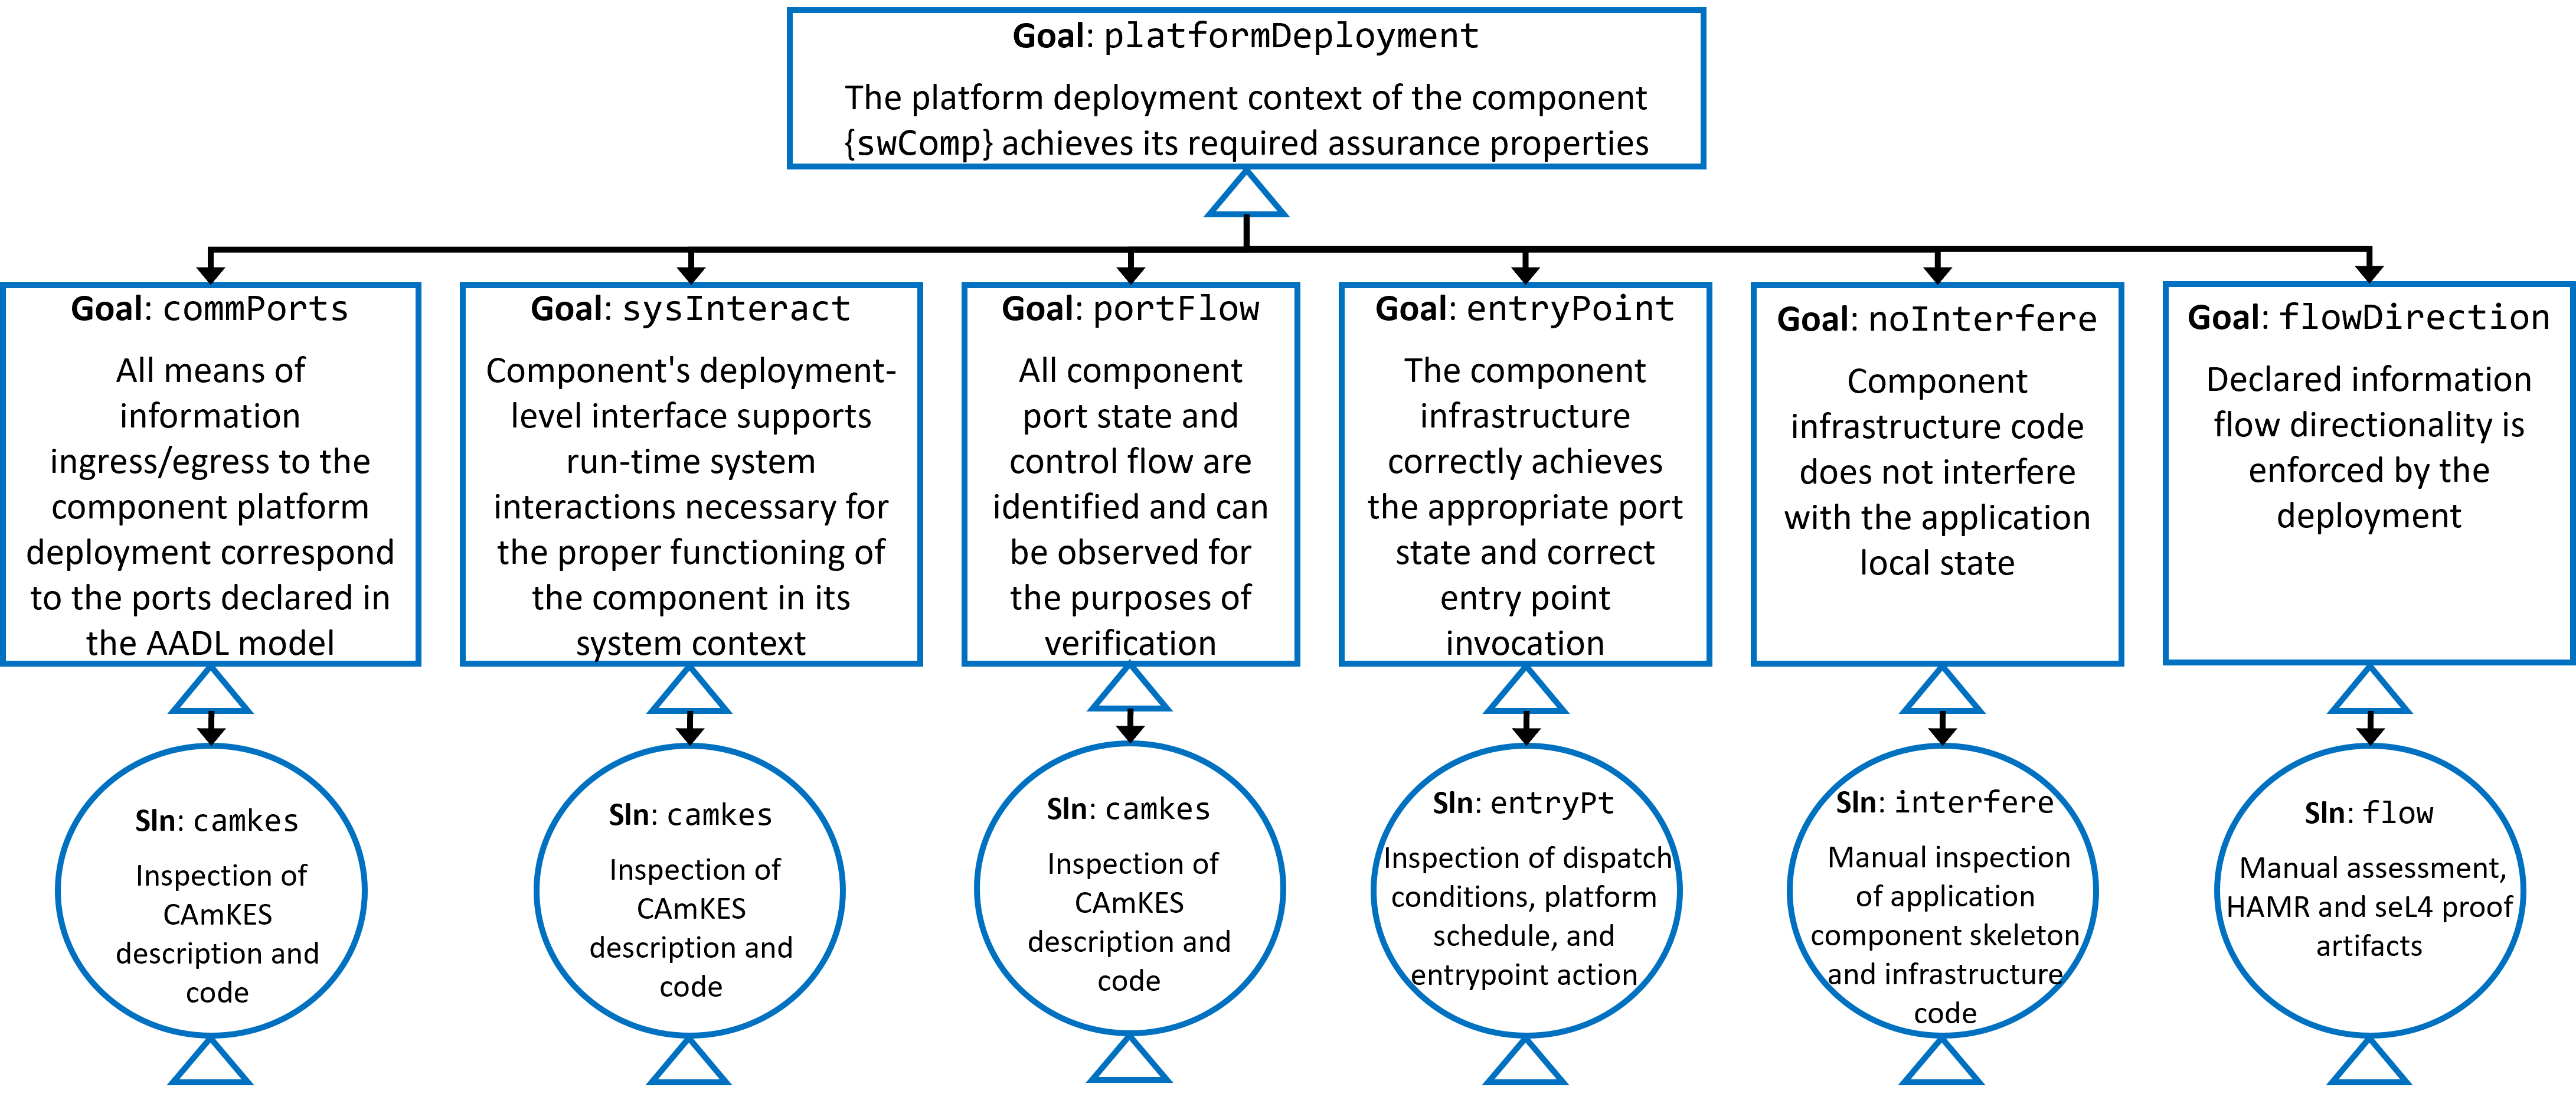
\includegraphics[width=\textwidth]{figs/platform-deployment-context-achieves-assurance-properties.png}
	\caption{Assurance pattern for arguing platform deployment context achieves the required assurance properties.}
	\label{fig:platform-deployment-context-achieves-assurance-properties} 
\end{figure}



In addition to demonstrating that \textit{deployed} software components satisfy their requirements, we must also argue that the platform components guarantee their required properties and the system implementation preserves them.

\section{Conclusion}
\label{sec:conclusion}

In this paper, we have presented a collection of hierarchical cyber-resiliency assurance patterns, which are bundled with our BriefCASE framework and instantiated with a specific system under development.  Automated instantiation and evaluation of the patterns provides us with confidence that we have adequately analyzed the system for cyber vulnerabilities and addressed the corresponding cyber requirements in the system design \textit{and} implementation.
Although these patterns mainly correspond to the automated BriefCASE features that support the CASE workflow outlined in Fig.~\ref{fig:workflow}, BriefCASE is not necessarily required to use them; with minor alteration they can be applied to any tool chain that adheres to the workflow.

Unfortunately, it will rarely be the case that an entire high-assurance system can be developed in this fashion.  Not all cyber requirements can be mitigated by an automated model transformation.  Not all component implementations can be synthesized in a provably correct manner.  And not all evidential development artifacts can be automatically evaluated.
%
Although these assurance patterns provide confidence that (a) the CASE workflow was properly followed for a specific system development configuration and (b) the resulting deployable system is acceptably cyber-resilient, additional patterns are still necessary to support typical development efforts we see in practice today.  
%
Our cyber-resiliency patterns are structured hierarchically, enabling straight forward insertion of additional pattern fragments corresponding to new cyber vulnerability mitigations, processes, and workflows. 
We anticipate working towards filling these gaps on future research projects as well as with contributions from the wider security assurance community.

\section{Acknowledgment}
This work was funded by DARPA contract HR00111890001. The views, opinions and/or findings expressed are those of the authors and should not be interpreted as representing the official views or policies of the Department of Defense or the U.S. Government.

\bibliographystyle{splncs04}
\bibliography{biblio}

\end{document}
